\section{VMware} \label{section: VMware}

VMware is a company that specializes in developing technologies for virtualization and cloud computing. Its software products and services enable organizations to efficiently manage their IT infrastructure, improve performance, and reduce costs. VMware offers solutions for network virtualization, cloud management, digital workspace solutions, and security solutions.

\subsection{vSphere 6.5}
vSphere is VMware's virtualization software suite that allows you to create and manage virtual machines and computing environments, using a set of software tools and services. With vSphere, you can run multiple virtual machines on the same physical server, each running its own operating system and applications. vSphere includes many features and capabilities that help make virtualized environments more reliable, scalable, and performant, such as: 

\begin{itemize}
    \item \textbf{vSphere Web Client}: A web-based management interface. 
    \item \textbf{ESXi}: The bare metal hypervisor installed on your machines. 
    \item \textbf{vCenter}: A centralized management system for your vSphere environment.
    \item \textbf{vSAN}: A software-defined storage solution to create a distributed storage platform in vSphere.
    \item \textbf{NSX}: A software-defined networking solution for your vSphere environment.
\end{itemize}

\subsubsection{vSphere Web Client}
The \href{https://docs.vmware.com/en/VMware-vSphere/7.0/com.vmware.vsphere.vcenterhost.doc/GUID-A618EF76-638A-49DA-991D-B93C5AC0E2B1.html}{vSphere Client} is an application that enables administrators to manage and monitor VMware vSphere environments. It comes with a graphical user interface (GUI) and allows users to connect to VMware vCenter Server, which serves as a central management console for multiple VMware vSphere hosts.

Through the vSphere Client, administrators can create and modify virtual machines, manage storage, configure networking, and monitor system performance, among other things. Essentially, it provides a range of tools that enable users to manage virtual infrastructure components effectively.

In addition to the traditional Windows-based vSphere Client, there's also a web-based version called the vSphere Client (HTML5), which is designed to work seamlessly across different operating systems and devices, including desktops, laptops, and mobile devices. This new client offers a simplified interface, improved performance, and support for new features introduced in vSphere 6.5 and later versions.

\begin{figure}[H]
    \centering
    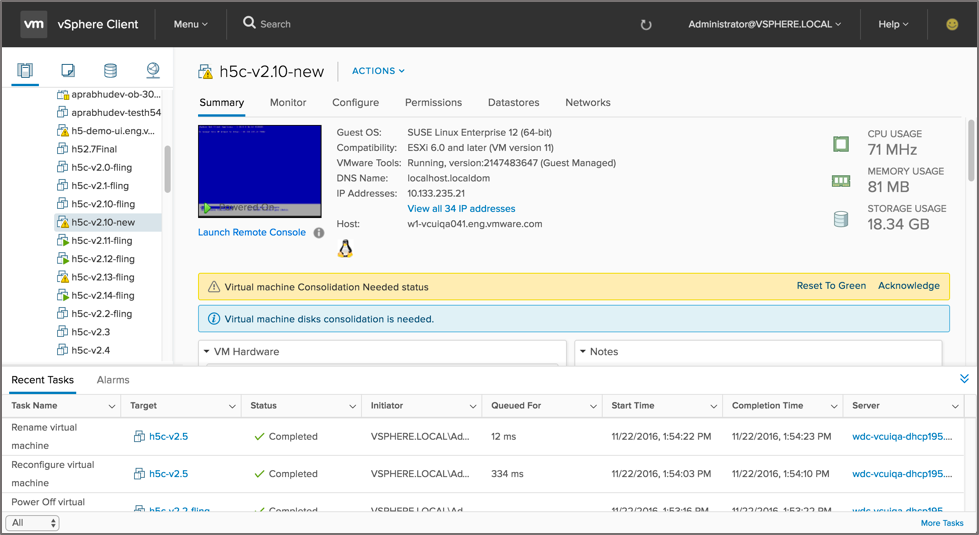
\includegraphics[scale = 0.9]{images/vsphere-client.jpg}
    \caption{vSphere Client \textcolor{red}{(STOLEN EXAMPLE)} }
    \label{vSphere Client}
\end{figure}

\subsubsection{ESXi}
VMware ESXi formerly known as ESX is a bare metal hypervisor that is installed directly on the physical server hardware and provides the ability to create, run, and manage virtual machines.

\begin{figure}[H]
    \centering
    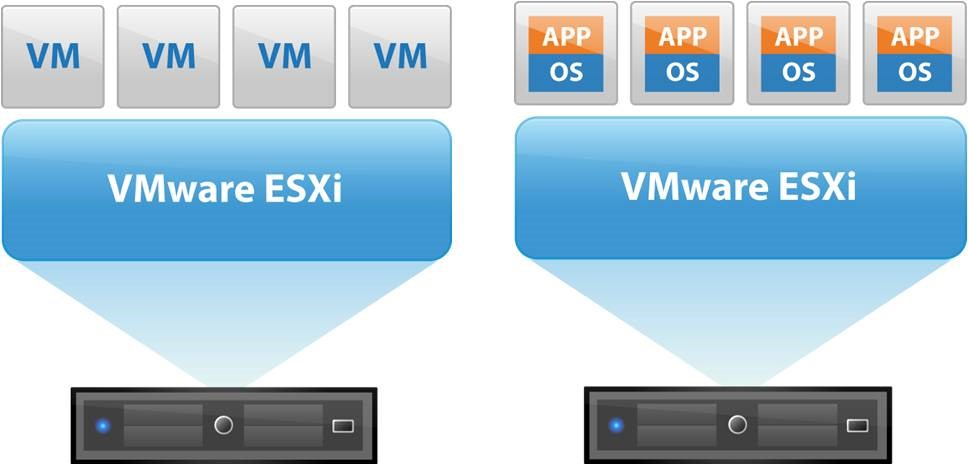
\includegraphics[scale = 0.55]{images/esxi.jpg}
    \caption{ESXi \textcolor{red}{(STOLEN EXAMPLE)} }
    \label{ESXi}
\end{figure}

\subsubsection{vCenter}
vCenter is a software platform developed by VMware that provides centralized management and control for their suite of virtualization products, including vSphere. Essentially, it allows you to manage multiple virtualized components from a single location, making it easier to manage complex virtualized environments.

With vCenter, you can manage hosts, clusters, virtual machines, networks, and storage resources in your virtualized environment. This includes advanced features like high availability, disaster recovery, and workload balancing, which help improve the reliability, availability, and performance of your virtualized infrastructure.

One of the biggest benefits of vCenter is that it provides advanced capabilities like automation, orchestration, and policy-based management. These features allow you to automate routine tasks, streamline operations, and enforce policies across your virtualized environment. Another key advantage of vCenter is that it enables you to manage large, complex virtualized environments at scale. By providing a single point of control, it simplifies management and reduces complexity, making it easier to manage many virtual machines and components.

\begin{figure}[H]
    \centering
    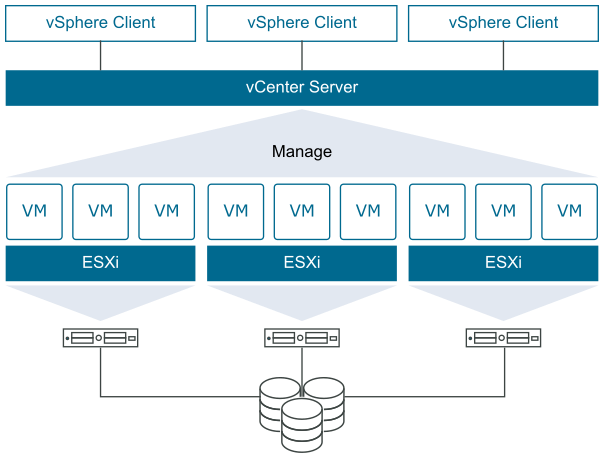
\includegraphics[scale = 0.65]{images/vmware-infrastructure-relationship.png}
    \caption{vCenter \textcolor{red}{(STOLEN EXAMPLE)} }
    \label{vCenter}
\end{figure}

\subsubsection{vSAN}
\href{https://docs.vmware.com/en/VMware-vSphere/7.0/com.vmware.vsphere.vsan-planning.doc/GUID-A80526C8-A941-4F84-9D44-D4B8B3914A95.html}{vSAN} is a software-defined storage solution developed by VMware, which allows organizations to create a distributed storage platform that is integrated with vSphere. This provides a highly scalable and available storage infrastructure, using standard hardware.

By creating a shared data store using the internal disks of ESXi hosts in a vSphere cluster, vSAN allows organizations to pool their storage capacity and performance into a single datastore, scaling it easily by adding more hosts to the cluster. vSAN features data replication, erasure coding, and automatic data rebalancing. Additionally, it offers advanced storage services such as deduplication, compression, and encryption, ensuring optimal storage efficiency and security which streamlines storage management, automates routine tasks, and helps to optimize storage utilization and cost savings.

\begin{figure}[H]
    \centering
    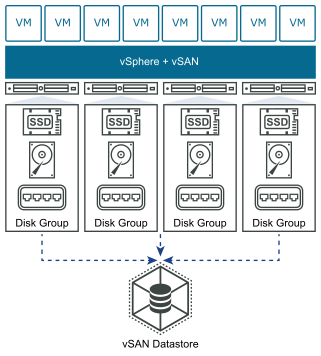
\includegraphics[scale = .8]{images/vsan-deployment.png}
    \caption{Standard vSAN Cluster \textcolor{red}{(STOLEN EXAMPLE)} }
    \label{vSan}
\end{figure}

\subsubsection{NSX}
\href{https://docs.vmware.com/en/VMware-NSX/index.html}{NSX} is a network virtualization and security platform created by VMware that provides a software-defined networking (SDN) solution that enables organizations to virtualize their network infrastructure, creating a more flexible, scalable, and manageable network.

NSX allows for all network components in your infrastructure to be virtualized, decoupling your network from existing hardware. This abstraction enables organizations to pool and automate network resources, which can reduce the time and cost of deploying and managing network infrastructure. NSX also offers advanced security features and networking capabilities which allows administrators to apply precise policies to specific workloads or applications. For example, NSX provides: network automation, multi-cloud and on-premises support, network segmentation, minimal cost and resource overhead, switching and routing, and load balancing features. 

\begin{figure}[H]
    \centering
    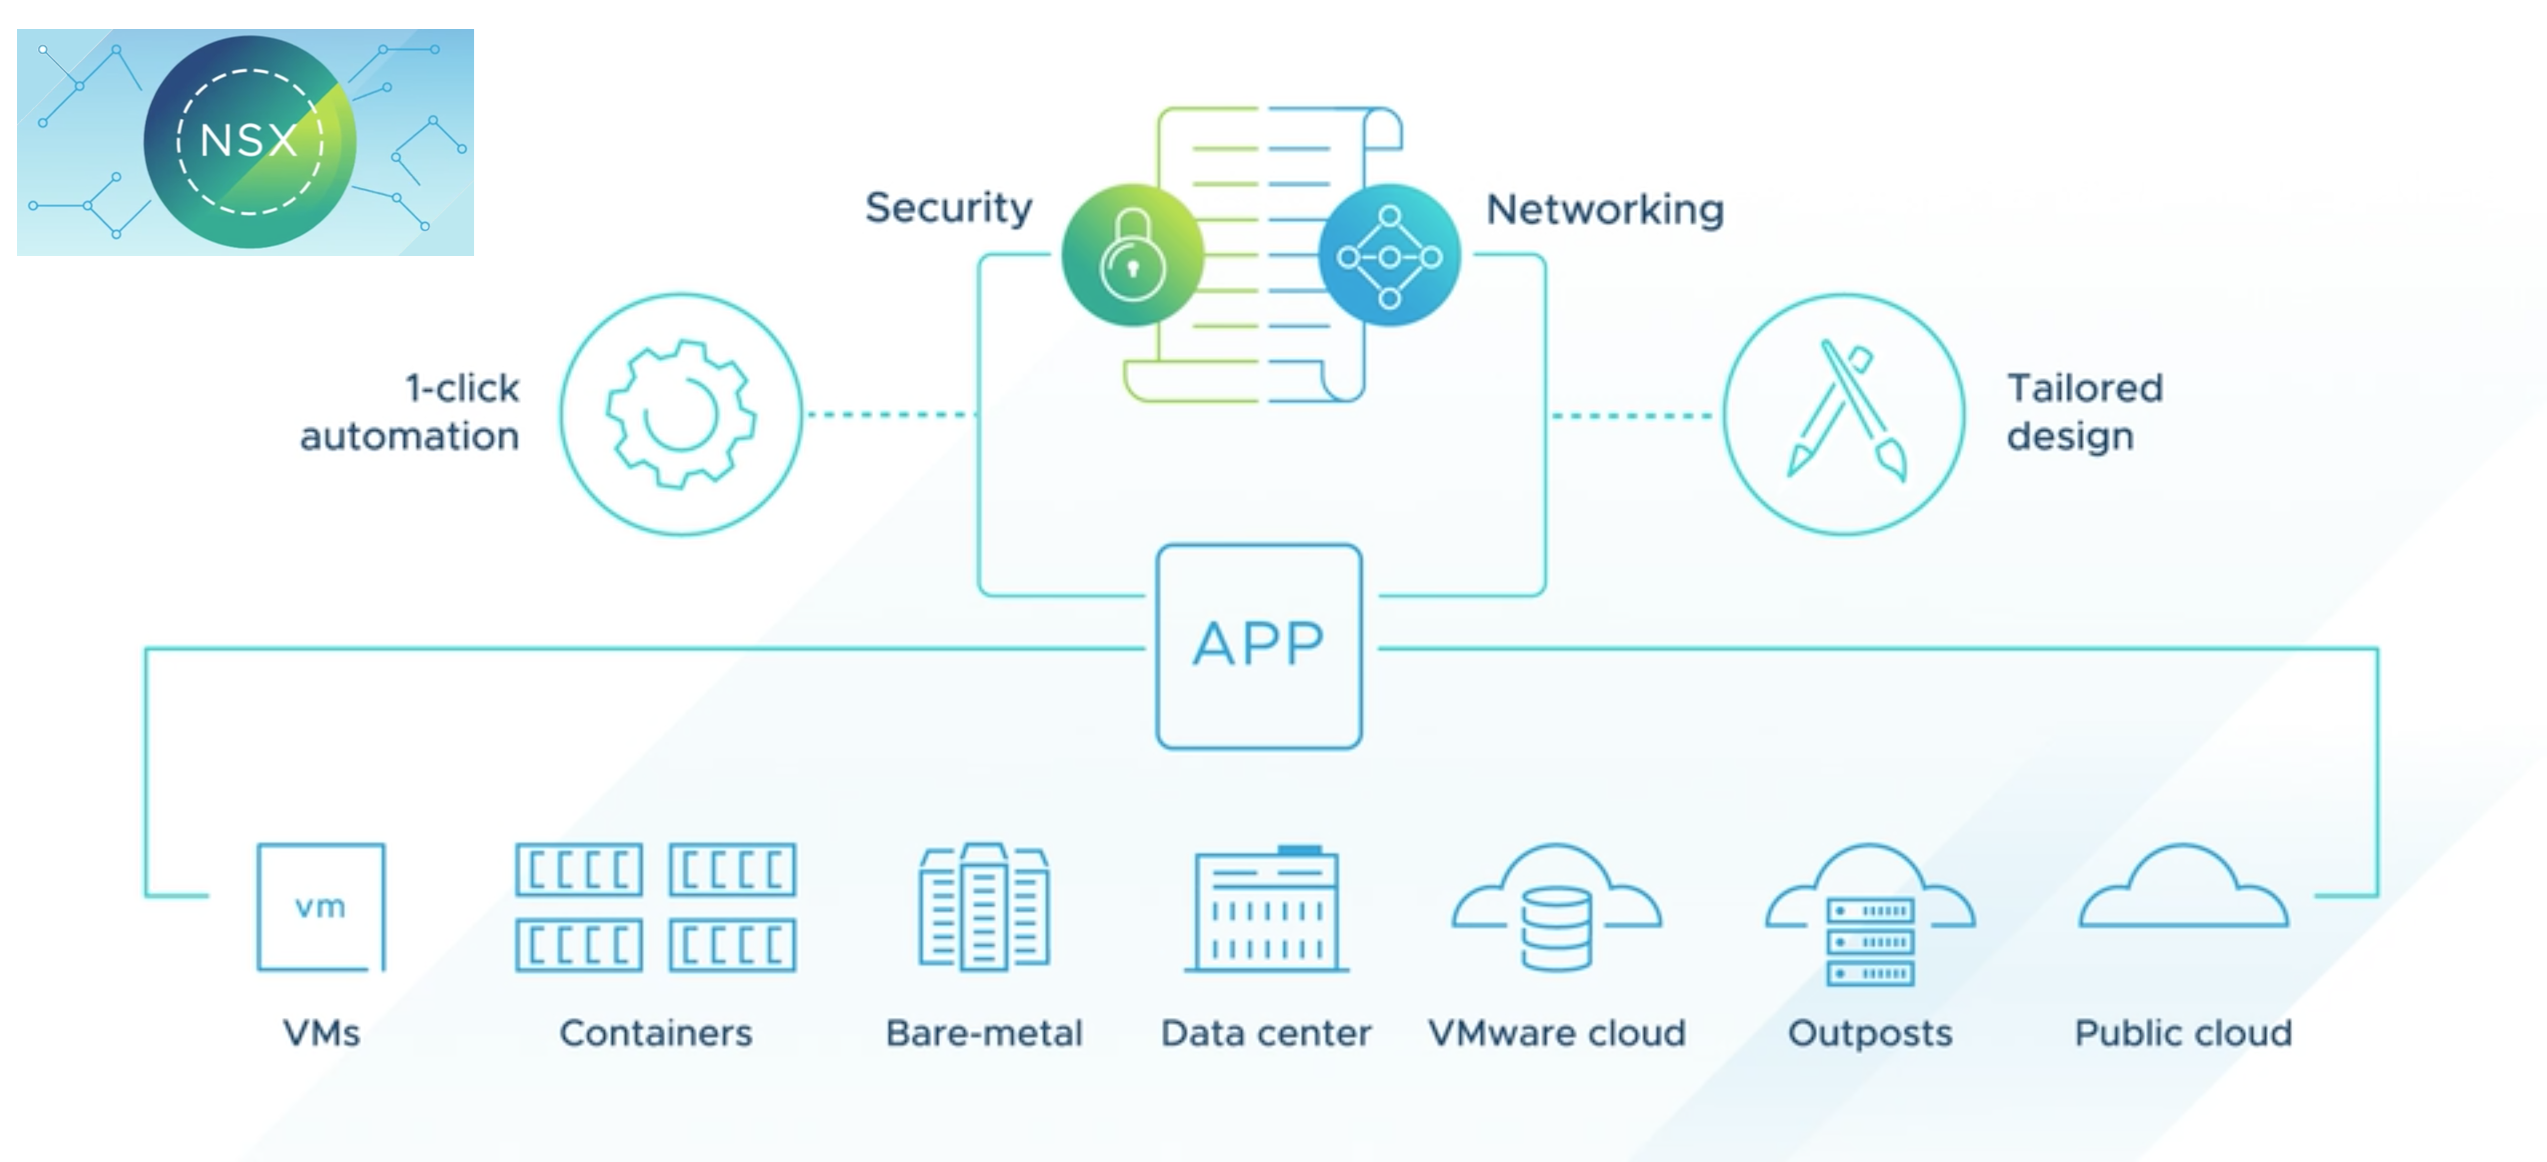
\includegraphics[scale = .19]{images/nsx-diagram.png}
    \caption{NSX Infrastructure \textcolor{red}{(STOLEN EXAMPLE)} }
    \label{NSX}
\end{figure}